\documentclass[../main.tex]{subfiles}

\begin{document}
	\chapter{Der Client}
	Der Client ist das Herzstück der entwickelten Anwendung. Er ist der Teil der Anwendung, welcher von den Endbenutzern/Endbenutzerinnen heruntergeladen und benutzt wird. Er ist das verbindende Glied zwischen den gespeicherten Informationen auf dem Server und den Benutzern/Benutzerinnen. Im folgenden Kapitel wird genauer auf die Funktionsweise des Clients eingegangen und seine Interaktionen mit dem Server beschrieben.
	
	\section{Betriebssystem und Programmiersprache}
	
	\subsection{Android}
	
	Der Client wurde für das Betriebssystem \emph{Android} entwickelt. Es wird ge"-schätzt, dass zwischen 85 und 86 Prozent aller heute verwendeten Mobiltelefone eine Version des Betriebssystems Android installiert haben. Dies macht Android zum mit Abstand meist verwendeten Betriebssystem für Mobiltelefone weltweit. Der Entscheid, die Studnetz-Applikation für Android Geräte zu entwickeln ist dadurch begründet, dass so die grosse Mehrheit der potentiellen Kunden/Kundinnen erreicht werden kann. \cite{android} %Die Entwicklung der Studnetz Applikation für Android Geräte macht also nur Sinn, da somit eine grosse Menge an Benutzern/Benutzerinnen erreicht werden kann. 
	
	Android basiert auf einem stark modifizierten Linux Kernel. Programme werden darauf in einer sogenannten \emph{Android Runtime} Umgebung ausgeführt. Diese Umgebung ist in der Lage, Bytecodes im \emph{Dex-Format} (Dalvik Executable-Format) auszuführen. Diese Dex-Formate werden dabei meist aus für die \emph{Java Virtual Machine} (JVM) kompilierten Bytecodes übersetzt. Die meisten Applikationen für Android wurden deshalb lange in der Programmiersprache Java programmiert, erst vor wenigen Jahren begann ein langsamer ein Umschwung zur neueren Programmiersprache \emph{Kotlin}, die jedoch auch in Bytecodes für die JVM kompiliert wird. Kotlin gewinnt hauptsächlich wegen seiner konzeptionell schönen Syntax an immer grösserer Beliebtheit, wobei insbesondere in der Entwicklung von Applikationen immer mehr auf Kotlin anstelle von Java gesetzt wird. \cite{androidJava}
	
	Die Studnetz-Applikation ist dennoch in Java programmiert worden, da ich als Entwickler mit dieser Sprache bereits vor dieser Arbeit schon gearbeitet habe und die Entwicklung von Mobilapplikationen mit Java Online sehr gut Dokumentiert ist. %\cite{bytecode}
	
	\subsection{Java}
	Für die Entwicklung der Studnetz Applikation wurde die Programmiersprache Java gewählt, da sie sehr gut dokumentiert ist und ich, als Entwickler, bereits vor dieser Arbeit Erfahrungen mit Java gesammelt hatte. Java ist eine Sprache der 3. Generation und gehört zu den objektorientierten Programmiersprachen. Sie wurde erstmals 1995 von Sun Microsystems veröffentlicht und ist seit 2010 in Besitz von Oracle. Java zeichnet sich besonders durch seine Plattformunabhängigkeit aus und eignet sich daher gut für kleinere Applikationen, die auf vielen verschiedenen Geräten funktionieren sollen.
	
	In der entwickelten Applikation wird die Sprache Java hauptsächlich für die logischen Prozesse verwendet, die hinter der optischen Benutzeroberfläche ablaufen.
	
	\subsection{XML}
	Für das Layout der Benutzeroberfläche des Clients wird für gewöhnlich nicht Java verwendet. Stattdessen weicht man auf die Auszeichnungssprache \emph{XML} aus. XML steht für \emph{Extensible Markup Language} und kann bis zu einem gewissen Grad mit HTML (\emph{Hypertext Markup Language}) verglichen werden, unterscheiden sich jedoch in einem zentralen Punkt. HTML wurde entwickelt, um zu bestimmen wie Informationen dargestellt werden. XML auf der anderen Seite setzt den Fokus auf die Informationen als solche selber, und weniger auf die Darstellung. Es ist jedoch trozdem möglich, auch XML für die Definition von Darstellungen zu verwenden, wie es beispielsweise bei Android Applikationen üblich ist. Weiter ist XML deutlich flexibler als HTML, da Entwickler/Entwicklerinnen mehr Möglichkeiten haben, eigene, neue Darstellungsformen zu definieren.
	
	Bei der Verwendung von XML in Android Applikationen wird XML verwendet, um zum einen die Layouts der darzustellenden Screen zu definieren, aber auch um statische Informationen wie beispielsweise zu verwendende Strings und Integer zu beschreiben. Somit können in einer Applikation auch relativ einfach verschiedene Sprachpakete integriert werden, da dafür lediglich alle definierten Strings, welche sich in einer Datei befinden, übersetzt werden müssen. Alle XML-Dateien zusammen bilden die \emph{Resources} einer Android Applikation. Diese Resources sind für die Java Klassen zugänglich und können durch diese manipuliert werden. Dies ermöglicht eine direkte Verknüpfung von Java mit dem Layout und ermöglicht die Entwicklung dynamischer Screens und Darstellungen. \cite{xml} \cite{xmlW3}
	
	\subsection{Android Studio}
	Die Entwicklung der Studnetz Applikation fand hauptsächlich innerhalb der Programmierumgebung \emph{Android Studio} statt. Android Studio ist eine von Google entwickelte Programmierumgebung (IDE) für die Entwicklung von Applikationen für Android Mobilgeräte und unterstützt alle dafür erforderlichen Sprachen. Die Umgebung bietet verschiedenste hilfreiche Werkzeuge für die Entwicklung von Applikationen zu. Dazu gehört beispielsweise ein Visueller Layout Editor, wo die Layouts sehr intuitiv via 'Drag and Drop' gestaltet werden können, wobei der dazu gehörige XML-Code im Hintergrund automatisch generiert wird. Zudem ist es möglich, entwickelte Applikationen sehr einfach auf lokalen Emulatoren zu testen, wobei in der Konsole von Android Studio dann allfällige Fehlermeldungen angezeigt werden. All dies und noch vieles mehr macht Android Studio zu einer sehr starken Programmierumgebung. Das Herunterladen und die Benutzung von Android Studio ist kostenlos. Die Wahl auf die Entwicklungsumgebung für die in dieser Arbeit entwickelten Applikation war sehr schnell gefällt, da es kaum vergleichbare Alternativen zu Android Studio gibt, zumindest was die Entwicklung von Android Applikationen anbelangt.
	
	\section{Klassenübersicht des entwickelten Clients}
	Im folgenden Abschnitt wird auf den entwickelten Client auf einer technischeren Ebene eingegangen. Es ist an dieser Stelle anzumerken, dass für diesen Abschnitt gewisse Grundkenntnisse des objektorientierten Programmierens und der Programmiersprache Java vorausgesetzt werden. Weiter ist anzufügen, dass die ab hier verwendeten Zeilenangaben innerhalb der Code Beispiele sich jeweils ausschliesslich auf die abgebildeten Ausschnitte des Codes beziehen und nicht die eigentlichen Zeilen im Sourcecode repräsentieren. Ebenfalls sind teilweise Stellen aus dem abgebildeten Sourcecode weggelassen worden. Diese Stellen sind dann durch das Symbol \emph{[...]} in der Abbildung gekennzeichnet.
	
	%Eine schematische Übersicht des den gesamten Clients ist in Abbildung \ref{clientOverview} dargestellt. Dort sind die einzelnen Activities und Fragments dargestellt und wie sie untereinander verknüpft sind.
	
	\subsection{Activities} \label{activities}
	Der Begriff \emph{Activities} ist Android spezifisch und beschreibt einen einzelnen Screen innerhalb einer Applikation. Innerhalb der Studnetz-Applikation werden sechs solche Activities verwendet. Zu jeder Activity gehört jeweils ein XML-Layout und eine Java-Klasse. Das XML-Layout bildet dabei die View-Komponenten, während die Java-Klasse die Presenter-Komponente bildet (siehe Kapitel \ref{mvp}). Auf die Struktur einer solchen XML-Layout-Datei wird hier nicht weiter eingegangen. Screenshots der fertigen Layouts finden sich in Kapitel \ref{studnetzApplikation}, wie die dazugehörigen XML-Dateien angesehen werden können wird in Kapitel \ref{github} beschrieben. Stattdessen wird der Fokus auf die Java-Klasse gelegt. Ein beispielhaftes Grundgerüst einer solchen Activity findet sich in Abbildung \ref{activityStructure}.
	
\begin{code}
	\begin{center}
		\begin{minted}[breaklines, mathescape, linenos, tabsize = 5]{java}
public class ActivityName extends AppCompatActivity {
			
	@Override
	protected void onCreate(Bundle savedInstanceState) {
		super.onCreate(savedInstanceState);
		setContentView(R.layout.ActivityLayoutName);
		
		[...]	
	}
	
	@Override
	protected void onStart() {
		super.onStart();
		
		[...]
	}
	
	@Override
	public boolean onOptionsItemSelected(MenuItem item) {
		
		[...]
		
		return super.onOptionsItemSelected(item);
	}
}	
		\end{minted}
		\caption{Grundgerüst einer Activity}
		\label{activityStructure}
	\end{center}
	
\end{code}

	Alle dargestellten Funktionen sind optional und müssen deshalb nicht zwangsweise in einer Activity vorkommen. Sie werden jedoch in der Studnetz-Applikation so gut wie immer benutzt.

	\paragraph{Die onCreate-Methode}
	Die \emph{onCreate}-Methode in den Zeilen drei bis acht ist die Kernfunktion einer jeden Activity. Sie ist die erste Funktion die in einem Lebenszyklus einer Activty ausgeführt wird und definiert das zu verwendende XML-Layout (Zeile 7). Anschliessend folgen meist die Instantiierungen der einzelnen, für die Activity relevanten Objekte. Dazu gehören zum einen rein Java seitige Objekte wie zum Beispiel ein Objekt der Klasse \emph{UserModel} (siehe Kapitel \ref{models}) aber es werden auch bestimmten Komponenten der View wie beispielsweise Schaltflächen passende Listener-Klassen zugewiesen. Diese Objekte erlauben es, die dazugehörige View zu manipulieren und ihnen neue Eigenschaften zuzusprechen.

	\paragraph{Die onStart-Methode}
	Die \emph{onStart}-Methode in Zeile 12 bis 15 ist die zweite Methode, die im Lebenszyklus einer Activity ausgeführt wird. Zum Zeitpunkt, bei welcher sie ausgeführt wird, ist der Screen für den Benutzer/die Benutzerin bereits sichtbar. In ihr werden meist diese Prozesse ausgeführt, die ansonsten zu grösseren Verzögerungen beim Laden einer Activity führen würden. Ein Beispiel hierfür wäre das Laden eines Profilbildes oder andere mit dem Server verknüpfte Prozesse.
	
	\paragraph{Die onOptionsItemSelected-Methode} 
	\sloppy
	Die \emph{onOptionsItemSelected}-Me"-tho"-de in den Zeilen von 19 bis 24 wird dann ausgeführt, wenn eine Schaltfläche in der Toolbar eines Screens betätigt wurde. In ihr wird dann jeweils definiert, was bei der Betätigung einer Schaltfläche geschehen soll. Dies kann zum Beispiel ein Wechsel zu einer neuen Activity sein oder das Ändern zu einem anderen Fragment.
	\fussy
	
	\subsection{Fragments}
	\emph{Fragments} sind ebenfalls Android spezifische Elemente und sind mit Activities vergleichbar. Gleich wie Activities bestehen sie sowohl aus eine Java-Presenter wie einer XML-View. Der grosse Unterschied ist jedoch, das Fragments im Gegensatz zu Activities keine eigenständige Screens sind, sondern jeweils innerhalb einer Acitvity eingebettet werden. Sie besitzen dann dort einen vorgegebenen Rahmen in welchem ihr Layout angezeigt wird. Die zum Layout gehörenden Methoden finden sich in der dazugehörigen Java-Klasse. Eine Abbildung eines Grundgerüstes eines solchen Fragments findet sich in Abbildung \ref{fragmentStructure}.
	
	\begin{code}
		\begin{center}
			\begin{minted}[breaklines, mathescape, linenos, tabsize = 5]{java}
public class FragmentName extends Fragment {
			
	@Override
	public void onAttach(Context context) {
		super.onAttach(context);
		this.mActivity = (ParentActivityName) context;
		
		[...]
	}
	
	@Override
	public View onCreateView(LayoutInflater inflater, ViewGroup container, Bundle savedInstanceState) {
	
		View view = inflater.inflate(R.layout.FragmentLayoutName, container, false);

		[...]

		return view;
	}
			
	@Override
	public void onStart() {
		super.onStart();
	
	}
			
	@Override
	public boolean onOptionsItemSelected(MenuItem item) {
			
		[...]
			
		return super.onOptionsItemSelected(item);
	}
}	
			\end{minted}
			\caption{Grundgerüst eines Fragments}
			\label{fragmentStructure}
		\end{center}
		
	\end{code}

	\paragraph{Die onAttach-Methode}
	Die \emph{onAttach}-Methode (Zeile 3 bis 10) ist die erste Funktion im Lebenszyklus eines Fragments. In der entwickelten Applikation wird sie verwendet, um dem Fragment eine Referenz zur momentanen Applikationsumgebung (\emph{Context}) zu geben, in welcher sich die Parent-Activity befindet (Zeile 6). Dieses Objekt wird für diverse Prozesse benötigt, die auf Ressourcen der Applikation zugreifen müssen oder anderweitig mit dem Gerät interagieren.\cite{context}
	
	\paragraph{Die onCreateView-Methode}
	Die \emph{onCreateView}-Methode in den Zeilen 13 bis 20 ist nach der onAttach- und der onCreate-Methode die dritte Methode im Lebenszyklus eines Fragments. Die onCreate-Methode wird in den Fragments der Studnetz selten verwendet, weshalb sie hier nicht selber aufgeführt ist. Stattdessen übernimmt die onCreateView-Methode die Aufgabe des Definierens der View (Layout) und der wichtigen Objekte. Dabei wird zuerst in Zeile 15 ein neues Layout der Klasse \emph{View} instantiiert. Über dieses Objekt kann dann auf die einzelnen View-Komponenten des Layouts zugegriffen werden. Schlussendlich wird die fertig konfigurierte View in Zeile 19 zurückgegeben, wo sie dann für das Fragment als Layout verwendet wird.
	
	\paragraph{Die onStart-Methode}
	Die \emph{onStart}-Methode eines Fragments ist direkt vergleichbar mit der onStart-Methode einer Activity. Gleich wie in einer Activity wird die onStart-Methode ausgeführt, wenn das Layout des Fragments bereits sichtbar ist. Auch sie wird für vom Server abhängige Prozesse verwendet, bei welchen mit Verzögerungen zu rechnen ist.
	
	\paragraph{Die onOptionItemSelected-Methode}
	Auch bei der \emph{onOptionItemSelected}-Methode kann auf die äquivalente Methode der Activites in Kapitel \ref{activities} verwiesen werden, da die Hauptaufgabe der Methode das Definieren der Aktionen in der Toolbar ist.
	
	\subsection{Models} \label{models}
	Der Begriff \emph{Models} beschreibt eine Reihe von Klassen, die hauptsächlich für das strukturierte Speichern von Informationen innerhalb des Clients verwendet werden und bilden somit die Model-Komponenten des Systems (siehe Kapitel \ref{mvp}). Die Models der Studnetz Applikation können generell vom Aufbau her in in vier Abschnitte unterteilt werden:
	
	\begin{itemize}
		\item Die \emph{Felder} eines Models: Die Felder, auch \emph{Member Variables} genannt, sind der Datenspeicher eines Models. Sie werden meist als erstes innerhalb der Klasse in Forme einer Reihe von Variablen definiert. \cite{memberVariables}
		\item Die \emph{Konstruktoren}: Die Konstruktoren befinden sich meist an zweiter Stelle. Über sie wird das Model initialisiert. Dabei kann es durchaus mehrere verschiedene Konstruktoren innerhalb eines Models geben. Ihnen werden meist über die Parameter  Daten mitgegeben, die für die Felder benötigt werden.
		\item  Die \emph{Getter}- und die \emph{Setter}-Methoden: Die Getter- und die Setter-Methoden finden sich als letzte in einem Model und sind die Methoden, die anderen Klassen den Zugriff auf die Felder des Models erlauben. Dabei können über die Setter-Methoden, auch \emph{Mutator Methods} genannt, die Felder nachträglich verändert werden, während über die Getter-Methoden, auch \emph{Accessor Methods} genannt, der Inhalt eines bestimmten Feldes abgerufen werden kann. \cite{accessorsAndMutators}
	\end{itemize}

	\subsubsection{Das UserModel}
	Das UserModel-Model ist das Model, in welchem die Informationen eines einzelnen Benutzerprofils gespeichert werden. Hierzu findet sich ein Feld für alle dafür relevanten Werte. Bei der Initialisierung wird unterschieden, ob das Model das Model des Clientbenutzers/der Clientbenutzerin selber ist oder ob es sich um ein fremdes Profil handelt. Entsprechend sind Informationen wie Passwort oder Email nicht immer innerhalb des Models gesetzt. Eine Abbildung eines Konstruktors des Models findet sich in Abbildung \ref{userModelConst}.
	
	\begin{code}
	\begin{center}
		\begin{minted}[breaklines, mathescape, linenos, tabsize = 5]{java}
		
	
public userInfo(int id, String username, String name, String firstname, [...], String temp_profilepicture_path, String JSON) {
	this.id = id;
	this.JSON = JSON;

	this.username = username;
	this.name = name;
	this.firstname = firstname;
	this.school = school;
	this.grade = grade
	this.description = description;
	
	this.french = french;
	this.spanish = spanish;
	this.english = english;
	this.music = music;
	this.chemistry = chemistry;
	this.biology = biology;
	this.maths = maths;
	this.physics = physics;
	this.german = german;
	
	this.passwordHash = passwordHash;
	this.salt = salt;

	this.temp_profilepicture_path = temp_profilepicture_path;
}
		\end{minted}
		\caption{Konstruktor der UserModel-Klasse}
		\label{userModelConst}
	\end{center}
	
\end{code}
	Das UserModel ist das zentralste Model der entwickelten Applikation. Es wird in allen Activities und Fragements mit Ausnahme des Logins und der Registrierung verwendet. Da jedoch das UserModel-Objekt selber nicht zwischen den Acitivties weitergegeben werden kann, wird hierzu ein JSON-String verwendet, der im Konstruktor auf Zeile 3 gesetzt wird. Der dabei verwendete JSON-String ist der gleiche, der der Ergänzungsfach-Server verwendet, wenn er Benutzerinformationen an den Client schickt.
	
	\subsubsection{Das ProfilePictureModel}
	Für das Darstellen und Speichern von Profilbild auf dem Client wird das ProfilePictureModel-Model verwendet. Das Model besitzt Felder für die drei verschiedenen Formate, in welchen ein Profilbild innerhalb der Applikation auftreten kann.
	
	\begin{itemize}
		\item Das \emph{Bitmap}-Format: Das Bitmap-Format ist das Format, welches von Android für die Darstellung von Bildern verwendet wird. Es wird in der Applikation verwendet, um das anzuzeigende Bild der \emph{ImageViews} (XML-Objekt für das Darstellen von Bildern) zu definieren.
		\item Das \emph{Base64}-Format: Base64 ist das Bild-Format welches für den Transfer einer Bilddatei zwischen Server und Client verwendet wird. Wie bereits in Kapitel \ref{MySQLStructure} erwähnt ist es ebenfalls das Format, in welchem die Bilder in der Datenbank gespeichert werden.
		\item Die temporäre \emph{Cache}-Datei: Die temporäre Cache-Datei ist eine Datei im lokalen Cache-Speicher des Gerätes. Cache-Speicher wird verwendet um temporär benötigte Dateien zu speichern, damit sie nicht immer wieder erneut geladen werden müssen. Jede Applikation auf einem Gerät besitzt dabei ihr eigenes Cache-Verzeichnis. Innerhalb der entwickelten Applikation werden jeweils für geladene Profilbilder Cache-Dateien erstellt. Ab dann werden die Bilder jeweils nur noch über den Pfad zur Cache-Datei referenziert. Dies macht einen einfachen Transfer der Bilder von Activity zu Activity möglich. \cite{cache}
	\end{itemize}

	Das ProfilePictureModel-Model kann dabei über jedes der drei Formate initialisiert werden, weshalb es jeweils einen Konstruktor für jedes Format besitzt. Anschliessend wird das gegebene Format in die anderen Formate übersetzt. Hierzu finden sich eine Reihe von Methoden in der ProfilePictureModel-Klasse. Hinzu kommtein vierter Konstruktor, der das Objekt mithilfe einem Parameter der Klasse \emph{Uri} initialisiert. Uri (Uniform Resource Identifier) ist eine Form der Dateireferenzierung. Sie wird bei der Auswahl eines neuen Profilbildes verwendet und kann ebenfalls in die anderen Formate umgewandelt werden. Eine Abbildung der Felder und der Konstruktoren findet sich in Abbildung \ref{profilePictureModelConst}.
	
\begin{code}
	\begin{center}
		\begin{minted}[breaklines, mathescape, linenos, tabsize = 5]{java}
public class ProfilePictureModel {

	private static final int MAX_QUALITY = 100;

	private boolean success = false;
	private Context mContext;
	private Bitmap imageBitmap;
	private String BASE64, path;
	private File tempFile;

	public ProfilePictureModel(Context context, String BASE64) {
		this.mContext = context;
		this.BASE64 = BASE64;
		this.imageBitmap = decodeBASE64(this.BASE64); //Methode für das Umwandeln von Base64 zu Bitmap
		createTemp(this.imageBitmap, MAX_QUALITY); //Erstellen einer neuen Bild-Datei im Cache
		this.success = true;
	}

	public ProfilePictureModel(Context context, Bitmap imageBitmap) {
		[...]
	}

	public ProfilePictureModel(Context context, Uri imageUri, int quality) {
		[...]
	}

	public ProfilePictureModel(Context context, File tempFile) {
		[...]
	}
	
	[...]
}
		\end{minted}
		\caption{Felder und Konstruktoren der ProfilePictureModel-Klasse}
		\label{profilePictureModelConst}
	\end{center}
	
\end{code}

	Eine weitere Aufgabe des ProfilePictureModel-Models ist die Regulierung der Bildqualität und Auflösung. Dies ermöglicht, dass egal was für ein Bild ein Benutzer/Benutzer als Profilbild ausgewählt hat, alle Bilddateien ungefähr gleich gross sind und der gleichen Auflösung entsprechen. Zudem werden die Bitmaps innerhalb der Applikation jeweils in einer runden Form dargestellt. Diese wird ihnen innerhalb des ProfilePictureModel-Models gegeben, wobei hierzu jedoch auf ein bereits existierendes Github-Repository von Arthur Teplitzki \cite{Cropper}zurückgegriffen wurde, welches verschiedene Tools für das Zuschneiden von Bildern bietet. Dieses Repository wird noch etwas mehr in Kapitel \ref{imageCropping} thematisiert.
	
	\subsubsection{Das ChatModel}
	Das \emph{ChatModel}-Model ist das simpelste Model der Studnetz Applikation und wird für die Chats verwendet. Im Model befinden sich Felder für die wichtigsten Kernangaben eines Chats wie die UserModel-Models von beiden Chatparteien, eine Firebase-Referenz zu den Firebase-Profilen beider Chatparteien sowie die Firebase-Referenz zum Chat selber. Eine Abbildung des einzigen Konstruktors sowie den Felder findet sich in Abbildung \ref{chatModelConst}.
	
\begin{code}
	\begin{center}
		\begin{minted}[breaklines, mathescape, linenos, tabsize = 5]{java}
public class ChatModel {

	private UserModel mMainprofileModel, mUserprofileModel;
	private DatabaseReference mMainprofileRef, mUserprofileRef, mChatRef;

	public ChatModel(UserModel mMainprofileModel, UserModel mUserprofileModel, DatabaseReference mMainprofileRef, DatabaseReference mUserprofileRef, DatabaseReference mChatRef) {
		this.mMainprofileModel = mMainprofileModel;
		this.mUserprofileModel = mUserprofileModel;
		this.mMainprofileRef = mMainprofileRef;
		this.mUserprofileRef = mUserprofileRef;
		this.mChatRef = mChatRef;
	}
}

		\end{minted}
		\caption{Felder und Konstruktor der ChatModel-Klasse}
		\label{chatModelConst}
	\end{center}
	
\end{code}
		
	%\subsection{Requests}
	\subsection{Auflistungen mithilfe von RecyclerViews}
	In der Studnetz Applikation wird an mehreren Orten eine Form einer Auflistung von Elementen benötigt. Dies ist beispielsweise bei der Anzeige der gefundenen Suchergebnissen der Fall oder wenn die offenen Chats aufgelistet werden. Für das Darstellen einer solchen Auflistung werden gleich mehrere verschiedene Klassen benötigt.
	
	\subsubsection{Das XML-Layout eines Elementes}
	Standardmässig verwenden Listen für die einzelnen Elemente ein extrem simples Layout für die einzelnen Elemente. Oft reicht dies jedoch nicht aus sondern die Elemente sollen angepasster an ihre spezifische Aufgabe sein. Hierzu wird ein XML-Layout definiert, welches jeweils für ein Element der Liste verwendet werden soll. Ein Beispiel eines solchen Elementes findet sich in Abbildung \ref{listElement}.
	
	\begin{figure}
		\centering
		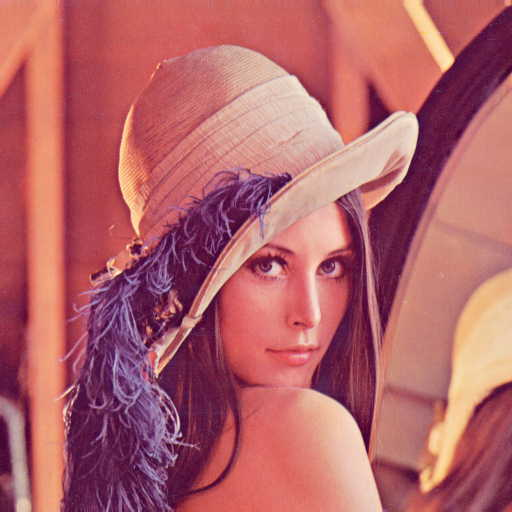
\includegraphics[width=\textwidth, height=\linewidth/2]{./images/lena.jpg}
		\caption{Einzelnes Element wie es bei der Auflistung der Suchergebnisse verwendet wird}
		\label{listElement}
	\end{figure}

	\subsubsection{Das Model eines Elements}
	Um den verschiedenen Elementen der Auflistung Informationen zuzuschreiben zu können, kommen Models zum Einsatz. Jedem Element wird ein Model zugeschrieben, welches die für das Element wichtigen Informationen beinhaltet. Wie solche Models aufgebaut sind wurde bereits in Kapitel \ref{models} beschrieben, weshalb hier nicht näher darauf eingegangen wird.
	
	\subsubsection{Die ViewHolder-Klassen}
	ViewHolder-Klassen beschreibt jeweils ein einzelnes Element der Auflistung. Innerhalb eines ViewHolders sind Dinge wie das zu verwendende Layout wie auch das zum Element gehörende Model referenziert. Es ist teilweise umstritten, wie weit der Aufgabenbereich der ViewHolder-Klasse einer Liste gehen soll. In der entwickelten Applikation hat der ViewHolder jeweils neben den bereits erwähnten Aufgaben auch die Aufgabe, das XML-Layout des Elementes auf die Informationen des Models anzupassen. Hierzu findet sich meist eine \emph{validate}-Methode, welche diese Modifikation der View ermöglicht. Ein Beispiel für eine solche ViewHolder-Klasse findet sich in Abbildung \ref{viewHolder}.

\begin{code}
	\begin{center}
		\begin{minted}[breaklines, mathescape, linenos, tabsize = 5]{java}
class ResultViewHolder extends RecyclerView.ViewHolder{
	
	private UserModel model;
	private View view;
	
	public ResultViewHolder(View view) {
		super(view);
		this.view = view;
	}
	
	public void validate(UserModel model) {
		this.model = model
	
		TextView name_tv = view.findViewById(R.id.result_name_textview);
		TextView school_tv = view.findViewById(R.id.result_school_textview);
		
		[...]
		
		name_tv.setText(this.model.getFirstname() + " " + this.model.getName());
		school_tv.setText(this.model.getSchool() + this.model.getStringGrade());
	}
	
	[...]
	
}
		\end{minted}
		\caption{ViewHolder-Klasse für die Auflistung der Suchergebnisse}
		\label{viewHolder}
	\end{center}
\end{code}

	%Bei der Darstellung einer Auflistung werden jeweils immer so viele ViewHolder-Objekte initialisiert, wie auf dem Bildschirm maximal sichtbar sein können. Daraufhin wird die validate-Methode für jeden ViewHolder aufgerufen, wobei ihr jeweils das dem Element zugewiesene Model als Parameter überreicht wird (Zeile 11). Wenn nun die Liste durchgesehen wird, bleibt die Anzahl der geladenen ViewHolder konstant. Es werden lediglich die nicht mehr sichtbaren ViewHolder wiederverwertet für die nun neu sichtbaren Elemente, wobei die validate-Methode des ViewHolders erneut mit einem anderen Model aufgerufen wird. Dieser Prozess wird als \emph{recycling} bezeichnet.
	
	\subsubsection{Die Adapter-Klassen}
	Adapter-Klassen haben die Aufgabe, die Elemente und somit auch die ViewHolder-Objekte einer Liste zu verwalten. Sie bestimmen, welcher Datensatz welchem Element zukommt und welche View für ein Element verwendet werden soll. In der entwickelten Applikation wird hierzu für die Auflistung der Suchergebnisse und der offenen Chats eine Subklasse der \emph{RecyclerView.Adapter}-Klasse verwendet, während für die Chats selber eine Subklasse der \emph{FirebaseRecyclerAdapter}-Klasse verwendet wird. Grundsätzlich ist der Aufbau beider Adapterarten vergleichbar. Der grosse Unterschied ist jedoch, dass FirebaseRecyclerAdapter über eine Referenz mit einer Firebase Echtzeitdatenbank verknüpft sind. Der Datensatz der Auflistung wird jeweils in Echtzeit mit der Datenbank synchronisiert. Auf den FirebaseRecyclerAdapter soll hier nicht weiter eingegangen werden. Stattdessen wird der Fokus auf den normalen RecyclerAdapter gelegt. Ein Beispiel eines solchen Adapters findet sich in Abbildung \ref{chatOverviewAdapter}.
	
\begin{code}
	\begin{center}
		\begin{minted}[breaklines, mathescape, linenos, tabsize = 5]{java}
class ChatoverviewAdapter extends RecyclerView.Adapter<OpenChatViewHolder>{

	private ChatoverviewFragment mFragment;
	private Map<Integer, OpenChatModel> mDataset;

	public ChatoverviewAdapter(ChatoverviewFragment mFragment) {
		this.mFragment = mFragment;
		this.mDataset = mFragment.getDataset();
	}

	@Override
	public OpenChatViewHolder onCreateViewHolder(ViewGroup parent, int viewType) {
		View view = LayoutInflater.from(parent.getContext()).inflate(R.layout.openchat, parent, false);
		OpenChatViewHolder viewHolder = new OpenChatViewHolder(view);
		return viewHolder;
	}

	@Override
	public void onBindViewHolder(OpenChatViewHolder holder, int position) {
		OpenChatModel model = mDataset.get(mDataset.keySet().toArray()[position]);
		holder.validate(model);
		holder.getView().setOnClickListener(new OnOpenChatListener(mFragment, model));
		holder.setProfilePicture(new ProfilePictureModel(mFragment.getActivity().getBaseContext(), new File(model.getUserModel().getTempProfilePicturePath())));
	}

	@Override
	public int getItemCount() {
		return mDataset.size();
	}
}
		\end{minted}
		\caption{RecyclerAdapter-Klasse für die Auflistung der offenen Chats}
		\label{chatOverviewAdapter}
	\end{center}
\end{code}

	Typisch für einen Adapter ist ein Feld für den darzustellenden Datensatz, welcher sich hier auf Zeile 4 in Form einer Map mit einem Integer als Key und einem OpenChatModel-Model als Wert findet. 
	
	Das OpenChatModel-Model ist wiederum ein sehr simples Model, welches nur für diese Auflistung verwendet wird. Es beinhaltet Felder für die benötigten Firebase-Referenzen und das Profil des Chatpartners in Form eines UserModel-Models. Zudem kommt noch einen String für die zuletzt im Chat geschickte Nachricht.
	
	Der Datensatz des Adapters wird jeweils bereits bei der Initialisierung des Adapters über die Parameter des Konstruktors auf Zeile 6 referenziert. Hier ist es wichtig zu unterscheiden, dass es sich um eine Referenz und nicht um einen Klon des Datensatzes handelt. Dies bedeutet, dass wenn sich der Datensatz ändern sollte, die Liste über eine notifyDatasetChanged-Methode aktualisiert werden kann, ohne dass der Datensatz dabei erneut übergeben werden muss.
	
	In den Zeilen 12 bis 24 finden sich die beiden Kernmethoden eines RecyclerAdapters.
	
	\paragraph{Die onCreateViewHolder-Methode}
	Die \emph{onCreateViewHolder}-Me"-tho"-de hat die Aufgabe, das Layout eines einzelnen Elements zu laden (Zeile 13) und ein neues ViewHolder-Objekt zu instantiieren (Zeile 14). Diese Methode wird jeweils so oft aufgerufen, wie Elemente auf dem Bildschirm des Gerätes maximal sichtbar sein können und geschieht deshalb gleich beim Start der Auflistung. Zu diesem Zeitpunkt unterscheiden sich die verschiedenen Elemente jedoch noch nicht und sehen alle gleich aus. Die Methode wird nach dem Start der Auflistung nicht mehr aufgerufen, selbst wenn die Liste durchgesehen wird und neue Elemente sichtbar werden müssen.
	
	\paragraph{Die onBindViewHolder-Methode}
	\sloppy
	Die \emph{onBindViewHolder}-Me"-tho"-de \newline wird jeweils für jeden ViewHolder der sichtbaren Elemente aufgerufen. Dabei wird den einzelnen ViewHolder-Objekten ihr Model über die validate-Methode zugewiesen (Zeile 21). Das zugewiesene Model wird dabei über die Position des Elementes innerhalb der RecyclerView bestimmt (Zeile 20). Im Falle der ChatoverviewAdapter-Klasse findet sich hier noch eine weiter Methode der ViewHolder-Klasse, die das Definieren eines zu verwendenden Profilbildes ermöglicht (Zeile 22).
	\fussy
	
	Die onBindViewHolder-Methode wird nach dem Start der View aufgerufen, wenn ein Element vom Bildschirm verschwindet und ein neues erscheinen muss. Es wird dann der ViewHolder des verschwundenen Elements genommen und sein Model wird über die validate-Methode durch ein neues Model ersetzt. Damit kann erreicht werden, dass mit einer nur geringen Anzahl an gleichzeitig geladener Layouts trotzdem beliebig grosse Datensätze effizient dargestellt werden können. Dieser Prozess der Wiederverwertung von nicht mehr sichtbarer Elemente wird als \emph{recycling} bezeichnet, was auch den Namen der beiden Superklassen RecyclerView.ViewHolder und RecyclerView.Adapter erklärt.
	
	%Ein solcher RecyclerAdapter besteht in der Regel aus einem Konstruktor (Zeile 8), über welchen das Datenset des Adapter bestimmt (Zeilen 12-16), und drei wichtigen Funktionen: der \emph{getItemCount} Funktion (Zeile 42), die die Menge an gespeicherten Elementen zurückgibt, der \emph{onCreateViewHolder} Funktion (Zeile 20), die einen neuen ViewHolder mit einem bestimmten Layout instantiiert und der \emph{onBindViewHolder} Funktion (Zeile 28), die einem ViewHolder einen Datensatz zuweist (Zeile 29), die View des ViewHolders entsprechend konfiguriert (Zeile 30-34) und der View eine onClickListener zuweist, die das Profil des dargestellten Benutzers/der dargestellten Benutzerin öffnet (Zeile 38). Im falle des Adapters der Suchergebnisse findet sich hier noch eine weitere Methode mit dem Namen \emph{refresh} (Zeile 46), die für das nachträgliche Einfügen der Profilbilder eine wichtige Rolle spielt, jedoch dazu mehr in Kapitel \ref{profilePictures}.
	
	\subsection{Utility-Klassen}
	\subsubsection{Die JSONtoInfo-Klasse}
	Die \emph{JSONtoInfo}-Klasse ist eine in der Applikation sehr oft verwendete Klasse. Sie ist in der Lage über eine \emph{createNewItem}-Methode aus einem JSON-Objekt, wie es vom Server erhalten wird, ein UserModel-Model zu instantiieren. Diese Datenkonversion ist von grossem Vorteil, da UserModel-Objekte nicht zwischen Activities weitergegeben werden können, jedoch der String eines JSON-Objektes schon. Somit wird zu Beginn einer Activity jeweils aus den Extras der String des JSON-Objektes entzogen, dieser zu einem JSON-Objekt gemacht und dieses wiederum zu einem UserModel-Objekt konvertiert. Ein Beispiel für eine solche Anwendung wird in Abbildung \ref{JSONtoInfoAnwendung} dargestellt.
	
\begin{code}
	\begin{center}
		\begin{minted}[breaklines, mathescape, linenos, tabsize = 5]{java}
mainprofileModel = new JSONtoInfo(getBaseContext()).createNewItem(new JSONObject(extras.getString("clientInfo")));			
		\end{minted}
		\caption{Instantiierung eines UserModel-Objektes aus den Extras}
		\label{JSONtoInfoAnwendung}
	\end{center}
\end{code}
	
	\subsubsection{Die TempFileGenerator-Klasse}
	Die \emph{TempFileGenerator}-Klasse wird verwendet, um aus einem Base64 String eines Bildes eine entsprechende Datei um Cache zu erstellen. Hierzu wird die \emph{getTempFilePath}-Methode verwendet. Sollte der Base64 String jedoch dem Wert 0 entsprechen oder nicht gesetzt sein (null), wird ein vordefiniertes Platzhalter Bild an Stelle einer Datei im Cache verwendet. Der Pfad zur Bilddatei wird dann jeweils über den Rückgabewert zurückgegeben.
	
	\subsubsection{Die ProfilePictureLoader-Klasse}
	Die \emph{ProfilePictureLoader}-Klasse wird verwendet, um mehrere Profilbilder gleichzeitig zu Laden. Dies wird bei der Darstellung von Auflistungen benötigt, wo mehrere Profile mit verschiedenen Profilbildern gezeigt werden. Dabei werden jeweils beim Start der Auflistungen die Profilbilder der ersten 20 Datensatzeinträge mithilfe der ProfilePictureLoader-Klasse geladen. Dann werden wenn noch ungeladene Profile gezeigt werden über die ProfilePictureLoader-Klasse die nächsten 20 Profilbilder geladen, bis schlussendlich, wenn alle Ergebnisse durchgesehen worden sind, alle Profilbilder geladen sind.
	
	\subsubsection{Die MyReader-Klasse und die SchoolMapper-Klasse}
	Diese beide Klassen sind für die Auflistung der Schulen und der dazugehörigen Schulstufen verantwortlich. Dabei werden die von der Applikation unterstützten Schulen im einen Spinner angezeigt und wenn eine Auswahl getroffen wurde, werden die Schulstufen der ausgewählten Schule im zweiten Spinner angezeigt. Die unterstützten Schulen sind dabei in einem Textdokument gespeichert und mit einer Zahl versehen, die die Schulstufen der Schule bestimmt. Es ist die MyReader-Klasse, die dieses Dokument zu lesen vermag und anschliessend die gelesenen Zeile als Liste zurückgibt. Die SchoolMapper-Klasse übernimmt das Handling der beiden Spinner. Eine Abbildung der SchoolMapper-Klasse findet sich in Abbildung \ref{schoolMapper}.
	
\begin{code}
	\begin{center}
		\begin{minted}[breaklines, mathescape, linenos, tabsize = 5]{java}
public class SchoolMapper {

	private Spinner schoolSpinner, gradeSpinner;
	Map<String, Integer> mMap;
	private Context mContext;

	public SchoolMapper(Context mContext, Spinner schoolSpinner, Spinner gradeSpinner) {
		this.mContext = mContext;
		this.schoolSpinner = schoolSpinner;
		this.gradeSpinner = gradeSpinner;
	}

	public Map<String, Integer> map(List<String> mData) {
		Map<String, Integer> mOut = new LinkedHashMap<>();

		for(int n = 0; n < mData.size(); n++) {
			String[] tempData = mData.get(n).split(":"); //Schulen sind jeweils durch ein ":" von ihrerer Schulstufe getrennt, zum Beispiel: "Kantonsschule Ausserschwyz:6"
			mOut.put(tempData[0], Integer.parseInt(tempData[1]));
		}
		
		return mOut;
	}

	public void startDisplay(String path){

		MyReader mReader = new MyReader(mContext);

		mMap = map(mReader.read(path));
	
		String[] keySet = mMap.keySet().toArray(new String[mMap.size()]);

		ArrayList<String> mSchools = new ArrayList<>();

		for(int n = 0; n < mMap.size(); n++) {
			mSchools.add(keySet[n]);
		}

		ArrayAdapter<String> schoolAdapter = new ArrayAdapter<String>([...], mSchools);
		schoolAdapter.setDropDownViewResource( android.R.layout.simple_spinner_dropdown_item);
		schoolSpinner.setAdapter(schoolAdapter);
		schoolSpinner.setOnItemSelectedListener(new AdapterView.OnItemSelectedListener() { [...] }
	}
}	
		\end{minted}
		\caption{Instantiierung eines UserModel-Objektes aus den Extras}
		\label{schoolMapper}
	\end{center}
\end{code}

	Beim Initialisieren der Klasse werden die Referenzen zu den beiden Spinnern über die Parameter des Konstruktors der Klasse überreicht (Zeile 7). Wenn die \emph{startDisplay}-Methode (Zeile 25) aufgerufen wird, werden die beiden Spinner konfiguriert. 
	
	Hierzu wird zuerst über die \emph{map}-Methode (Zeile 13) das Textdokument mithilfe der MyReader-Klasse gelesen und die gelesenen Schulen (Zeile 29) gemeinsam mit der zugehörigen Schulstufenanzahl in eine \emph{LinkedHashMap} gespeichert (Zeile 14). Eine LinkedHashMap ist fast identisch zu einer normalen HashMap, wo auch jeweils ein Key gemeinsam mit einem Wert gespeichert werden. Der einzige Unterschied findet sich hier, dass sich die Reihenfolge, in welcher die Elemente in die HashMap eingefügt worden sind, gespeichert wird. Diese HashMap kann dann als Datensatz für den Schulspinner verwendet werden (Zeile 39).

	In den Schulspinner wird ein Listener implementiert, welcher bei der Auswahl einer Schule dann auch den Stufenspinner der ausgewählten Schule entsprechend konfiguriert (Zeile 43).

	%\subsection{Beispielhafte Erläuterung der \emph{MainActivity}}
	%\subsubsection{Aufbau der Activity}
	%\subsubsection{Aufbau der Fragments}
	\subsection{Profilbilder und \emph{Image Cropping}} \label{imageCropping}
	Kein Profil ist heutzutage ein richtiges Profil ohne ein passendes Profilbild. Ein Profilbild hilft den Benutzern/Benutzerinnen zum einen sich von einer möglichst guten Seite zu zeigen und um schnell einen ersten Eindruck von anderen Benutzern/Benutzerinnen zu bekommen. Auch in der entwickelten Applikation ist es möglich, ein Profilbild zu bestimmen. Dabei ist es Benutzern/Benutzerinnen möglich, vom Speicher des Gerätes ein Bild auszuwählen und es auf das gewünschte Format zuzuschneiden oder direkt mit der Kamera ein neues Bild aufzunehmen. Für die Implementierung dieser Features wurde auf zwei öffentliche Github Repositories zurückgegriffen, da die eigene Programmierung dieser Funktionen den Rahmen dieser Arbeit gesprengt hätte. Die Lizenzen für beide Repositories finden sich im Anhang.
	
	Das erste Repository läuft unter dem Namen \emph{EasyImage} und ermöglicht ein einfaches Zugreifen und Auslesen von Bildern aus der Galerie, wie auch direkt von der Kamera \cite{EasyImage}. Jedoch wären die Bilder an diesem Punkt einfach in der Grösse und Form, wie sie auf dem Gerät gerade gespeichert sind. Dies ist für ein Profilbild höchst ungeeignet. Hier kommt das zweite Repository ins Spiel. Dieses trägt den Namen \emph{Android Image Cropper} und basiert auf dem 2013 erschienenen \emph{Cropper} von Edmodo Inc. \cite{Cropper} \cite{edmodo}. Dieses Repository bringt eine Reihe an Funktionen für das Zuschneiden und Anpassen von Bildern mit sich. Dieser Prozess des Zuschneidens wird auch \emph{Cropping} genannt, was auch den Namen des Repositories erklärt. Wählt ein Benutzer/eine Benutzerin ein Bild aus, wird dieser Cropper gestartet. Ein Screenshot davon findet sich in Abbildung \ref{cropperImage}. Der Benutzer/Die Benutzerin kann daraufhin den Bereich des Bildes auswählen, welcher er/sie als Profilbild verwenden möchte. Danach kann die Auswahl bestätigt werden und das Bild wird daraufhin zugeschnitten. Dabei wird auch gleich die Qualität und Grösse des Bildes auf ein einheitliches Mass reduziert. So ist jedes Bild in der Datenbank ungefähr ähnlich gross. Zudem wird jedes Profilbild in einer zweiten, deutlich kleineren Version gespeichert. Dieses wird für die Suchergebnisse und die Aufgelisteten Chats verwendet, wo teilweise gleich 20 Bilder gleichzeitig geladen werden müssen. Um dabei Leistung zu sparen gibt es demnach von jedem Profilbild eine Version, die zwar sehr klein in Grösse und niedrig in Qualität ist, jedoch für die kleinen Icons bei der Suche komplett ausreicht. Beide Bilder werden in der Datenbank in der user\_profilepictures Tabelle gespeichert (siehe auch Kapitel \ref{MySQLStructure}).
	
	\begin{figure}
		\centering
		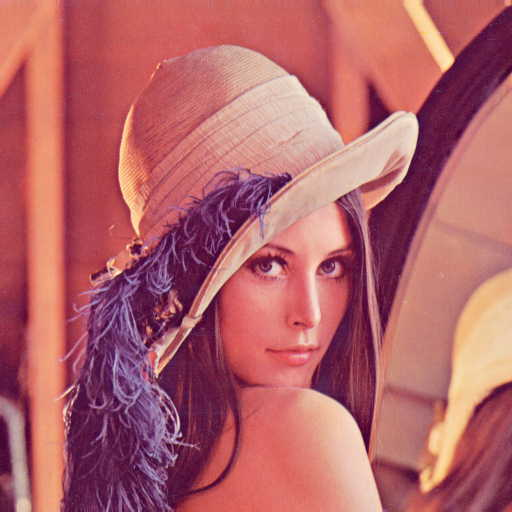
\includegraphics[width=\textwidth]{./images/lena.jpg}
		\caption{Screenshot des Croppers beim zuschneiden}
	\end{figure}
	
	\subsection{Interaktion mit dem Webserver (MySQL Datenbank)}
	Für Interaktionen mit dem Webserver, auf welchem sich auch die MySQL Datenbank befindet, wird auf die \emph{Volley}-Bibliothek zurückgegriffen. Die Volley-Bibliothek bietet diverse Tools für das effiziente Arbeiten mit Netzwerken und eignet sich für das Kontrollieren der Kommunikation mit dem Webserver auf Seiten des Clients. Die Kommunikation mit dem Webserver läuft dabei  in zwei Stufen ab: der Formulierung einer Anfrage und der Verarbeitung der Antwort.
	
	\subsubsection{Formulieren einer Anfrage}
	
	\paragraph{Die Request-Klassen}
	Eine \emph{Request}-Klasse definiert die Webadresse, an welche eine Anfrage gerichtet wird, sowie die dabei mitzugebenden Werte. Man kann sich als ein adressiertes Postpaket vorstellen, welches verschickt werden kann. Sie ist eine Subklasse der StringRequest-Klasse aus der Volley Library. Für jede Art der Anfrage muss jeweils eine eigene Request-Klasse erstellt werden, sie sind jedoch vom Aufbau her alle identisch. Ein Beispiel für eine solche Klasse findet sich in Abbildung \ref{requestKlasse}.
	
\begin{code}
	\begin{center}
		\begin{minted}[breaklines, mathescape, linenos, tabsize = 5]{java}
public class BigProfilePictureRequest extends StringRequest {

	private static final String URL = "http:// [...] /profilepicture_big_php.php";
	private Map<String, String> params;

	public BigProfilePictureRequest(int id, Response.Listener<String> listener) {
		super(Method.POST, URL, listener, null);
		params = new HashMap<>();
		params.put("user_id", id + "");
	}

	[...]
	
}
		\end{minted}
		\caption{Request-Klasse für die Anfrage nach einem Profilbild eines Benutzers}
		\label{requestKlasse}
	\end{center}
\end{code}

	Die Webadresse, an welche die Anfrage gehen soll, wird in einem der beiden Felder definiert (Zeile 3). Dabei wird angegeben, welches PHP-Skript aufgerufen werden soll. Das zweite Feld ist eine HashMap (Zeile 4). Die HashMap ist der Datencontainer für die zu übermittelnden Werte. Dabei sind im Falle des Beispiels der Key sowie der Wert der HashMap Strings. Die HashMap kann, nachdem sie erfolgreich an den Server übermittelt worden ist, verwendet werden, um die mitgegebenen Werte über die Keys wieder auszulesen.
	
	Der Konstruktor benötigt im Falle des Beispiels nur zwei Parameter: eine user\_id und ein Objekt der Klasse \emph{Response.Listener$<$String$>$} (Zeile 6). Daraufhin wird die Superklasse aufgerufen und die Anfragemethode, die URL, der ResponseListener (siehe Kapitel \ref{responseListener}) und ErrorListener als Parameter referenziert (Zeile 7). In der entwickelten Applikation wird immer die \emph{POST}-Methode für die Kommunikation zwischen Webserver und Client verwendet. Dann wird die user\_id als Wert in die HashMap eingefügt (Zeile 9).
	
	\paragraph{Das Stellen der Anfrage}
	Nachdem erfolgreich ein Objekt einer Request-Klasse instantiiert worden ist, kann die Request-Klasse über die sogenannte \emph{RequestQueue} aus der Volley Library als Anfrage an den Webserver gesendet werden. Ein Beispiel findet sich in Abbildung \ref{requestQueue}
	
\begin{code}
	\begin{center}
		\begin{minted}[breaklines, mathescape, linenos, tabsize = 5]{java}
BigProfilePictureRequest request = new BigProfilePictureRequest(mUserModel.getId(), new OnBigPictureResponseListener(this)); 		 //Instantiieren der Request-Klasse
RequestQueue queue = Volley.newRequestQueue(mActivity); //Instantiieren einer neuen RequestQueue
queue.add(request); //Das Stellen der Request-Klasse als Anfrage an den Server
		\end{minted}
		\caption{Request-Klasse für die Anfrage nach einem Profilbild eines Benutzers}
		\label{requestQueue}
	\end{center}
\end{code}	
	
	\subsubsection{Das Verarbeitung einer Antwort} \label{responseListener}
	\paragraph{OnResponseListener-Klasse} Die \emph{OnResponseListener}-Klasse ist einer Subklasse der Response.Listener$<$String$>$-Klasse der Volley-Bibliothek. Diese Listener-Klasse wird aufgerufen, wenn eine Antwort vom Server auf eine Anfrage empfangen wird. Die Antwort wird dabei in Form eines Strings übermittelt, der dann in ein JSON-Objekt umgewandelt werden kann. Ein Beispiel einer solchen Klasse findet sich in Abbildung \ref{OnResponseListener}.
	
\begin{code}
	\begin{center}
		\begin{minted}[breaklines, mathescape, linenos, tabsize = 5]{java}
class OnBigPictureResponseListener implements Response.Listener<String> {

	private OpenprofileFragment mFragment;
	private MainActivity mActivity;

	[...] //Konstruktor

	@Override
	public void onResponse(String response) {
		
		[...]

		JSONObject jsn = new JSONObject(response);
		boolean success = jsn.getBoolean("success");

		if (success) {
			[...]
		}
		[...]
	}
}
		\end{minted}
		\caption{OnBigPictureResponseListener-Klasse}
		\label{OnResponseListener}
	\end{center}
\end{code}		
	
	Bei einer empfangenen Antwort wird als erstes überprüft, ob die Aufgabe des PHP-Skriptes erfolgreich ausgeführt worden ist (Zeile 14 und 16). Je nachdem wird dann die Antwort weiter verarbeitet (Zeile 17) oder der Fehlschlag dem Benutzer/der Benutzerin mitgeteilt, sofern dies nötig ist (Zeile 19).
	
	\subsection{Interaktion mit der Firebase Echtzeitdatenbank}
	Die Interaktionen vom Client mit der Firebase Echtzeitdatenbank unterscheidet sich stark von der Interaktion mit dem Webserver. Anders als bei einem herkömmlichen Webserver ist das Implementieren von serverseitiger Datenverarbeitung in Form von Skripten sehr aufwändig und Firebase bietet hierzu kaum Tools. Deshalb wird bei der Arbeit mit Firebase Echtzeitdatenbanken oft sehr viel der Datenverarbeitung auf Seiten des Client gemacht. Dies bringt eine Menge potentieller Risiken in Bereichen Sicherheit mit sich, die jedoch im Rahmen dieser Arbeit in Kauf genommen worden sind. 
	
	\subsubsection{Verbindung (Wird erweitert sobald Sicherheit geklärt ist!)}
	Die Verbindung zum Server wird wie beim Webserver auch hier über eine Webadresse erstellt. Die Adresse wird dabei in einer separaten Datei definiert. Es ist auch in dieser Datei, wo die gesamten für die Authentifizierung benötigten Werte gespeichert sind. Die Authentifizierung wird dabei von Freibase selber geregelte und läuft über ein Google Konto.
	
	\subsubsection{Zugriff vom Client auf die Echtzeitdatenbank}
	Innerhalb des Clients wird über sogenannte \emph{Referenzen} auf den Server zugegriffen. Diese Referenzen sind im wesentlichen die Webadressen der verschiedenen JSON-Objekte. Über sie können neue Werte in die Datenbank eingefügt werden oder ausgelesen werden. Dieser Vorgang soll anhand zweier Beispiele demonstriert werden.
	
	\paragraph{Einfügen neuer Werte in die Firebase Echtzeitdatenbank}
	Das Einfügen neuer Werte in die Echtzeitdatenbank ist eher simpel. Ein Beispiel hierfür findet sich in Abbildung \ref{FirebaseWrite} wo ein Ausschnitt des Einfügens einer neuen Nachricht in einem Chat dargestellt ist.

\begin{code}
	\begin{center}
		\begin{minted}[breaklines, mathescape, linenos, tabsize = 5]{java}
final DatabaseReference newPost = mChatModel.getChatRef().child("Messages").push();
newPost.child("messageUser").setValue(messageUser);
		\end{minted}
		\caption{Einfügen von neuen Werten in die Firebase Echtzeitdatenbank}
		\label{FirebaseWrite}
	\end{center}
\end{code}
	
	Hierzu wird die zu verwendende Referenz definiert (Zeile 1). Über die \emph{getChatRef}-Methode des ChatModel-Models kann die Referenz zum Chat selber geholt werden. Über die \emph{child}-Methode wird zu einem JSON-Objekt mit dem Namen \emph{Messages} navigiert. Die \emph{push}-Methode bewirkt dann, dass ein neues JSON-Objekt mit einem zufällig generierten Namen erstellt wird. Diese nun konfigurierte Referenz kann verwendet werden, um neue Werte in die Datenbank einzufügen. Hierzu wird über die child-Methode ein neues JSON-Objekt erstellt, wo der einzufügende Wert über die \emph{setValue}-Methode eingefügt werden kann (Zeile 2). %Ein visualisierte Darstellung über diesen Vorgang findet sich in Abbildung \ref{FirebaseWriteVisualized}.
	
	\paragraph{Auslesen von Werten aus der Firebase Echtzeitdatenbank}
	Das Auslesen aus einer Firebase Echtzeitdatenbank ist im Gegensatz zum Einfüg"-en neuer Werte deutlich komplexer. Jedoch bietet Firebase für häufige Verwendungen wie zum Beispiel das Darstellen von Listen schon bestehende Interfaces und Klassen an, die diese Aufgabe weitgehend übernehmen. In Abbildung \ref{FirebaseRead} wird ein Code Ausschnitt dargestellt, der das Auslesen von Daten weitgehend selber bestimmt. Hierzu wird eine Klasse verwendet, in welche das \emph{ValueEventListener}-Interface implementiert wird. Diese Klasse wird für die Darstellung der offenen Chats benötigt, wo eine genauere Kontrolle über diesen Ladevorgang erforderlich ist.
	
\begin{code}
	\begin{center}
		\begin{minted}[breaklines, mathescape, linenos, tabsize = 5]{java}
class ChatsValueEventListener implements ValueEventListener {
	
	[...] //Konstruktor
	
	@Override
	public void onDataChange(DataSnapshot dataSnapshot) {
		[...]
	}

	[...]
}
		\end{minted}
		\caption{ValueEventListener-Klasse für das Auslesen von Daten aus der Firebase Echtzeitdatenbank}
		\label{FirebaseRead}
	\end{center}
\end{code}

\begin{code}
	\begin{center}
		\begin{minted}[breaklines, mathescape, linenos, tabsize = 5]{java}
[Firebase Reference].addValueEventListener(new ChatsValueEventListener(this));
		\end{minted}
		\caption{Zuweisung eines ValueEventListeners zu einer Referenz}
		\label{implementFirebaseRead}
	\end{center}
\end{code}
	
	Eine Klasse mit einem implementierten ValueEventListener-Interface kann jeweils einer oder mehreren Referenzen zugewiesen werden (siehe Abbildung \ref{implementFirebaseRead}). Hierzu wird innerhalb der Klasse bei der Zuweisung zu einer neuen Referenz und anschliessend immer wenn sich der Datensatz einer Referenz ändert die \emph{onDataChange}-Methode aufgerufen (Abbildung \ref{FirebaseRead}, Zeile 6). Diese bekommt über ihre Parameter einen sogenanntes \emph{DataSnapshot}-Objekt der Referenz. Ein solches DataSnapshot-Objekt ist eine Momentaufnahme aller im JSON-Objekt einer Referenz gespeicherten Werte. Diese Werte können dann innerhalb der onDataChange-Methode ausgelesen und weiter verarbeitet werden.
	
	Der grosse Vorteil dieser Art des Auslesens ist es, dass die Daten auf dem Client immer mit den Daten in der Firebase Echtzeitdatenbank synchronisiert werden.
	
	
	\section{Herunterladen des Projektes und der Applikation} \label{github}
	
\end{document}